\documentclass[12pt]{article}
\usepackage{geometry}                % See geometry.pdf to learn the layout options. There are lots.
\geometry{letterpaper}                   % ... or a4paper or a5paper or ... 
%\geometry{landscape}                % Activate for for rotated page geometry
\usepackage[parfill]{parskip}    % Activate to begin paragraphs with an empty line rather than an indent
\usepackage{daves,fancyhdr,natbib,graphicx,dcolumn,amsmath,lastpage,url}
\usepackage{amsmath,amssymb,epstopdf,longtable}
\usepackage[final]{pdfpages}
\usepackage{paralist}  % need to modify standard enumerate blocks
\usepackage{tabto}
\newcommand\mytab{\tabto{1cm}}
\DeclareGraphicsRule{.tif}{png}{.png}{`convert #1 `dirname #1`/`basename #1 .tif`.png}
\pagestyle{fancy}
\lhead{CE 3354 -- Engineering Hydrology}
\rhead{FALL 2025}
\lfoot{ES5}
\cfoot{}
\rfoot{Page \thepage\ of \pageref{LastPage}}
\renewcommand\headrulewidth{0pt}



\begin{document}
\begin{center}
{\textbf{{ CE 3354 Engineering Hydrology} \\ {Exercise Set 5}}}
\end{center}

\section*{\small{Exercises}}

\begin{enumerate}

\item a 50-acre single-family residential subdivision receives a rainfall intensity of 3 inches per hour for one hour.  The average runoff coefficient is 0.50.  Using a rational triangular hydrograph \footnote{Essentially apply the Modified Rational Method with $t_c$ equal to the storm duration} 

Determine:
    \begin{enumerate}[a)]
        \item Maximum (peak) discharge rate for the watershed.
        \item A plot of the discharge hydrograph in 6-minute intervals.
        \item The total volume of runoff from the subdivision for the entire storm.
    \end{enumerate}

\textbf{Solution(s):}
Entire problem as Jupyter Notebook (ENGR-1330) on following pages.
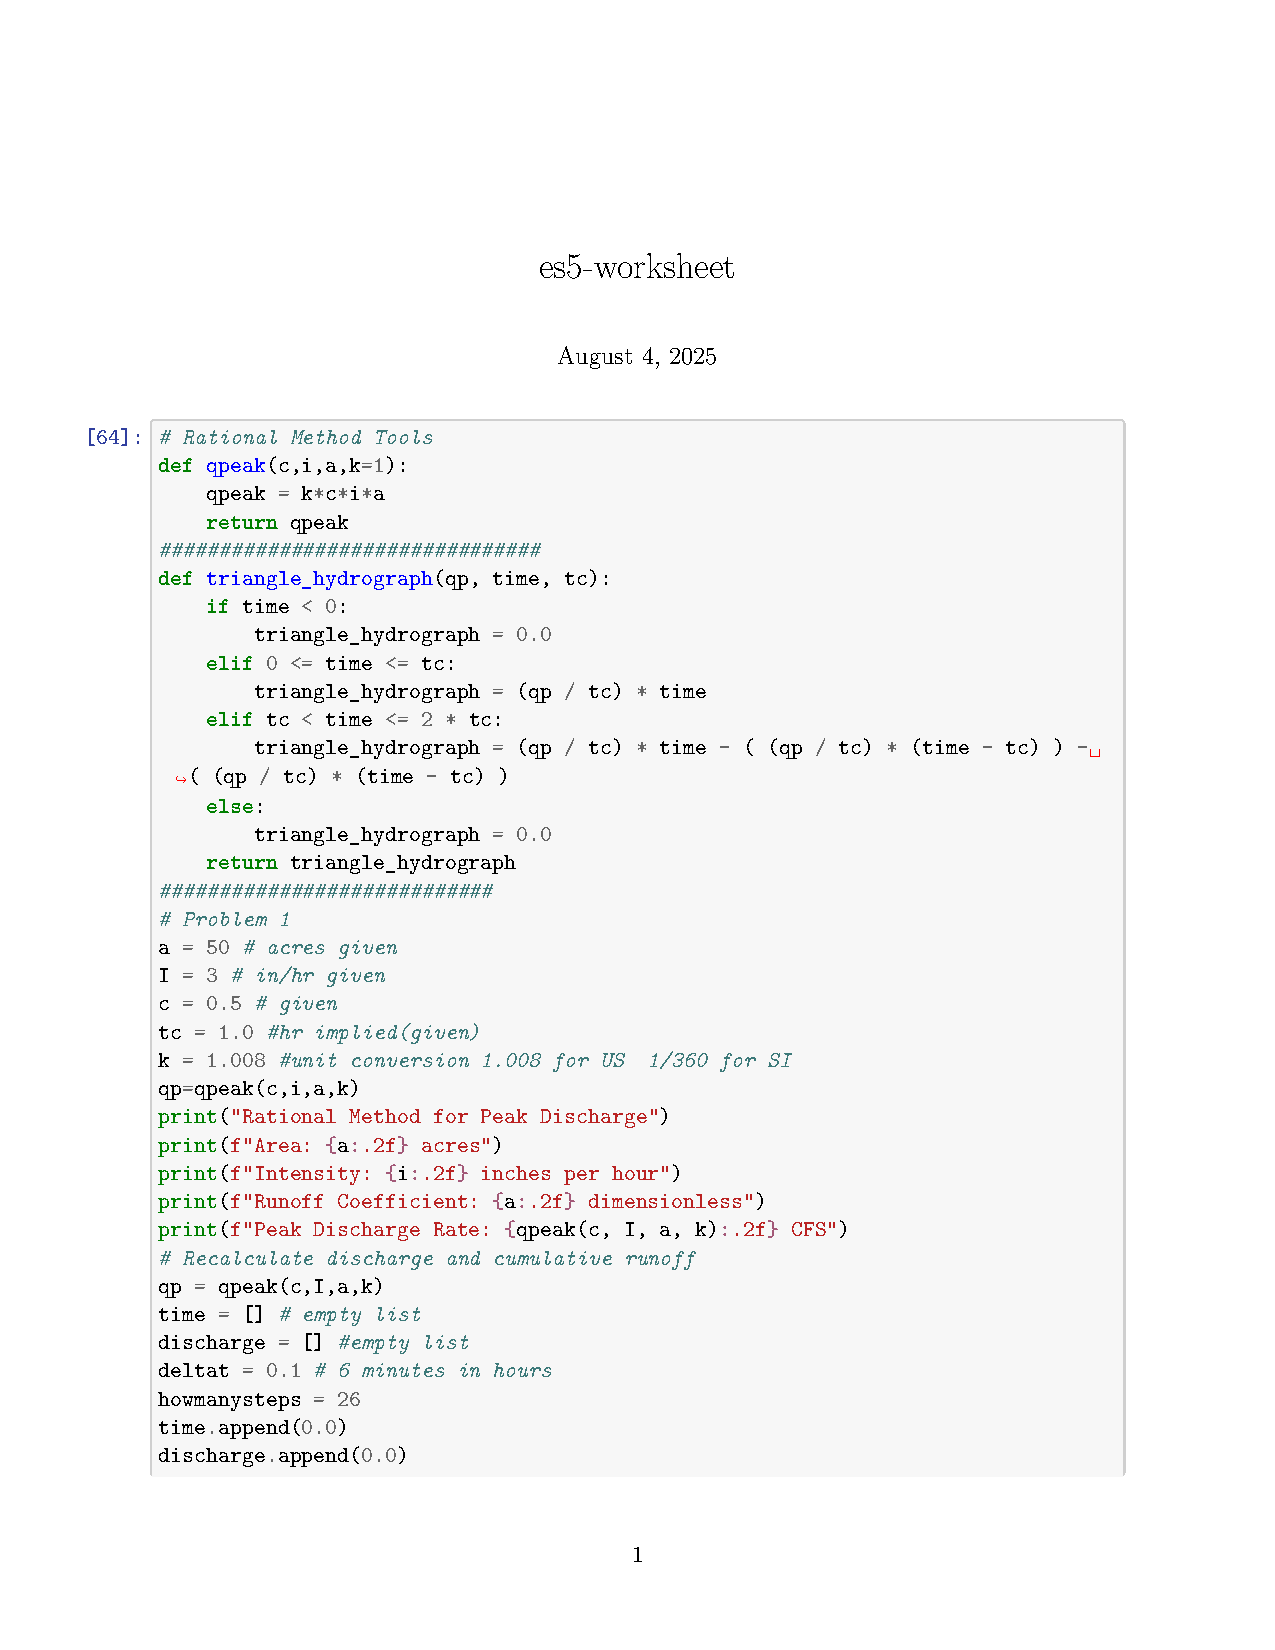
\includepdf[pages=-]{es5-ws1.pdf}

\clearpage

\item a 50-acre single-family residential subdivision receives a rainfall intensity of 3 inches per hour for one hour.  The average runoff coefficient is 0.50.  Using the NRCS triangular hydrograph \footnote{$t_c$ is set equal to the storm duration} 

Determine:
    \begin{enumerate}[a)]
        \item Maximum (peak) discharge rate for the watershed.
        \item A plot of the discharge hydrograph in 6-minute intervals.
        \item The total volume of runoff from the subdivision for the entire storm.
    \end{enumerate}

\textbf{Solution(s):}
Entire problem as Jupyter Notebook (ENGR-1330) on following pages.
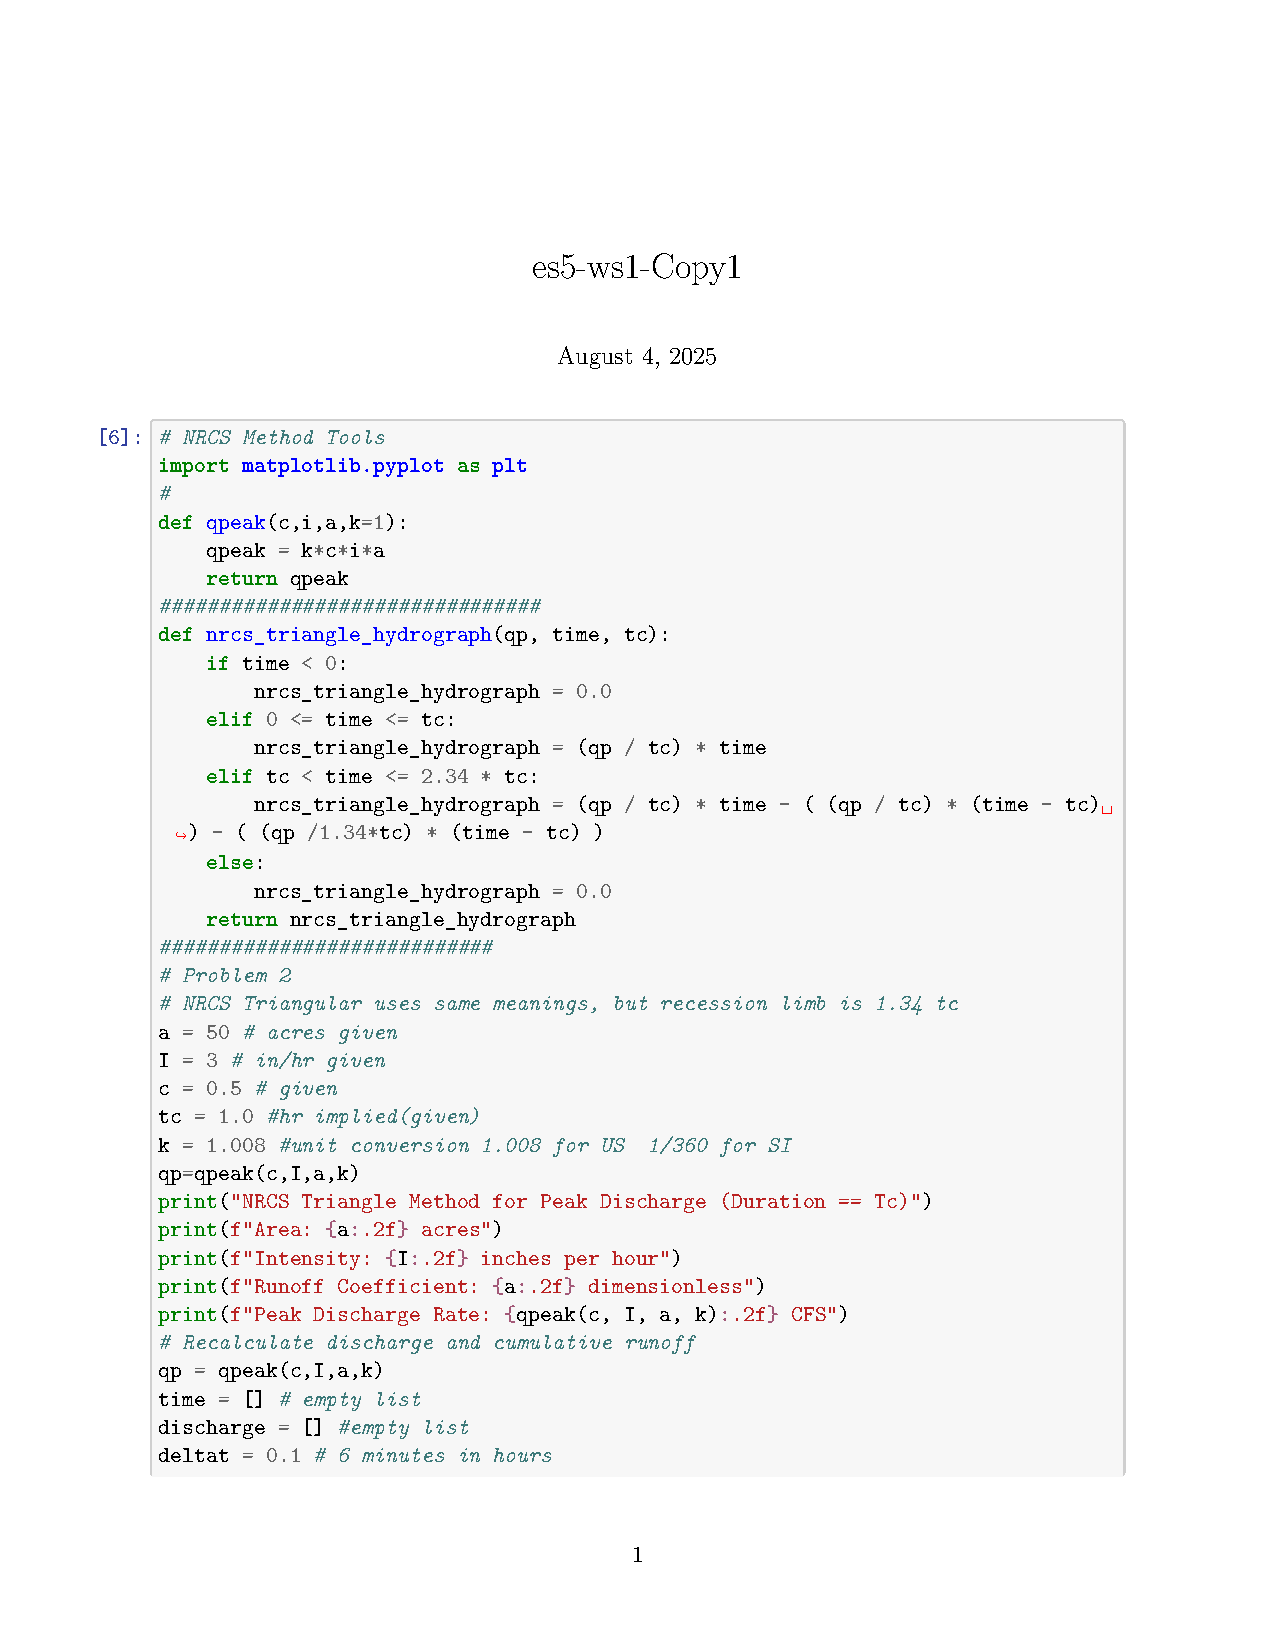
\includepdf[pages=-]{es5-ws2.pdf}

\clearpage

\item A watershed is comprised of sandy soil with a 500 foot path to an outlet.  The slope on that path is 5-percent.  The soil has a high water table limiting the potential watershed storage to 0.5 inches.  Using the NRCS Lag Equation method\footnote{\url{https://directives.nrcs.usda.gov/sites/default/files2/1712930818/31754.pdf}}

\begin{equation}
T_c = L^{0.8} \frac{(S_r + 1)^{0.7}}{1140 Y^{0.5}}
\end{equation}

%1900 in denominator replaced with 1140 in 2021 version

where: \\
\mytab $T_c$ = time of concentration, hr \\
\mytab $L$ = flow length, ft \\
\mytab $S_r$ = Potential storage (in.); $S_r = \frac{1000}{CN}-10$ \\
\mytab $CN$ = NRCS runoff curve number \\
\mytab $Y$ = average watershed slope, \% \\


Determine:
    \begin{enumerate}[a)]
        \item Time of concentration ($T_c$).
    \end{enumerate}

\textbf{Solution(s):}
Entire problem as Jupyter Notebook (ENGR-1330) on following pages.
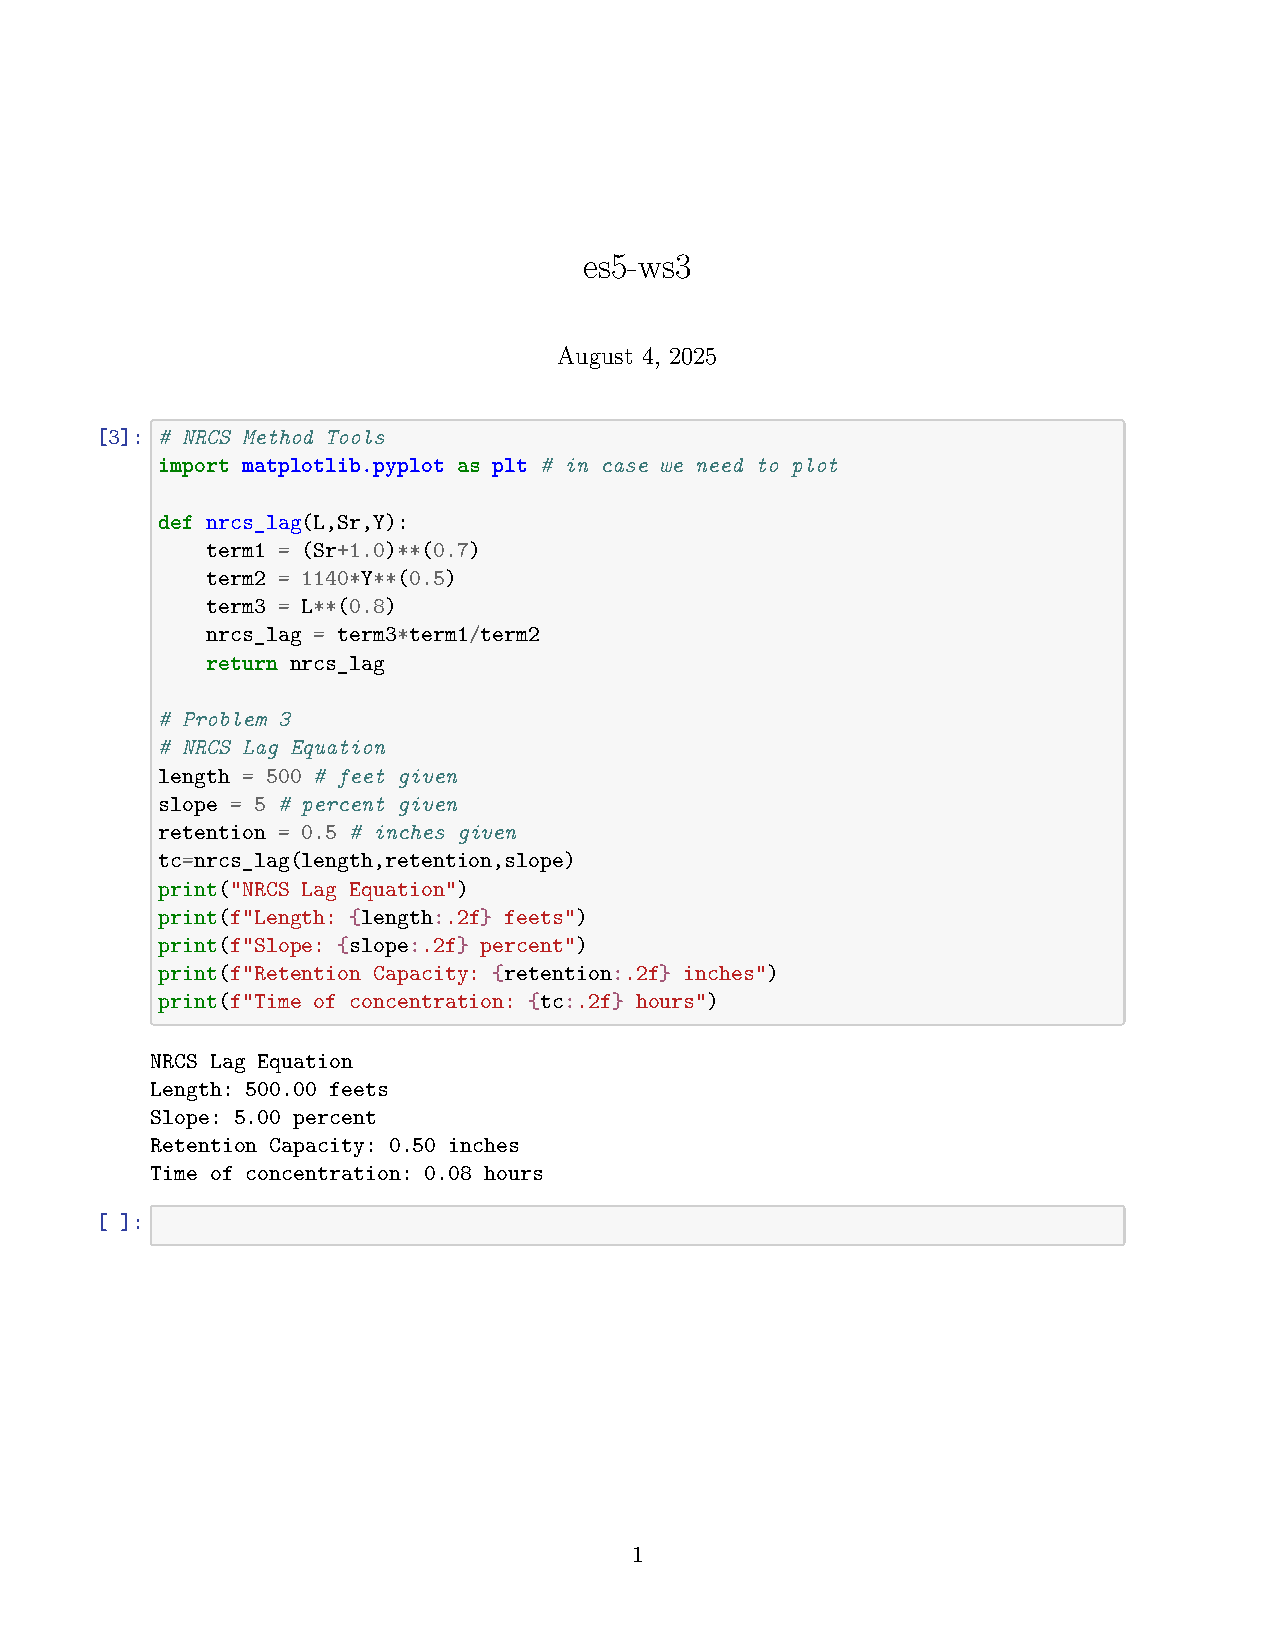
\includepdf[pages=-]{es5-ws3.pdf}

\clearpage

\item The runoff hydrograph below was produced by a 100 acre watershed.

\begin{table}[h!]
\centering
\caption{Somewhere USA Runoff Data}
\begin{tabular}{p{2.0in}p{2.0in}} % Column formatting, @{} suppresses leading/trailing space
~&~\\
Time (hours) & Runoff (CFS) \\
\hline
\hline
0.0 & ~0.0 \\
1.0 & 70.0 \\
2.0 & 160. \\
3.0 & 110. \\
4.0 & 80.0 \\
5.0 & 60.0 \\
6.0 & 45.0 \\
7.0 & 30.0 \\
8.0 & 20.0 \\
9.0 & 12.0 \\
10. & ~5.0 \\
11. & ~0.0 \\
\hline
\end{tabular}
\label{tab:SomewhereUSARain}
\end{table}

Determine:
    \begin{enumerate}[a)]
        \item Excess precipitation in watershed inches for the hydrograph.
        \item A unit hydrograph for the watershed.
        \item A plot of the unit hydrograph.
    \end{enumerate}

\textbf{Solution(s):}
Entire problem as Jupyter Notebook (ENGR-1330) on following pages.
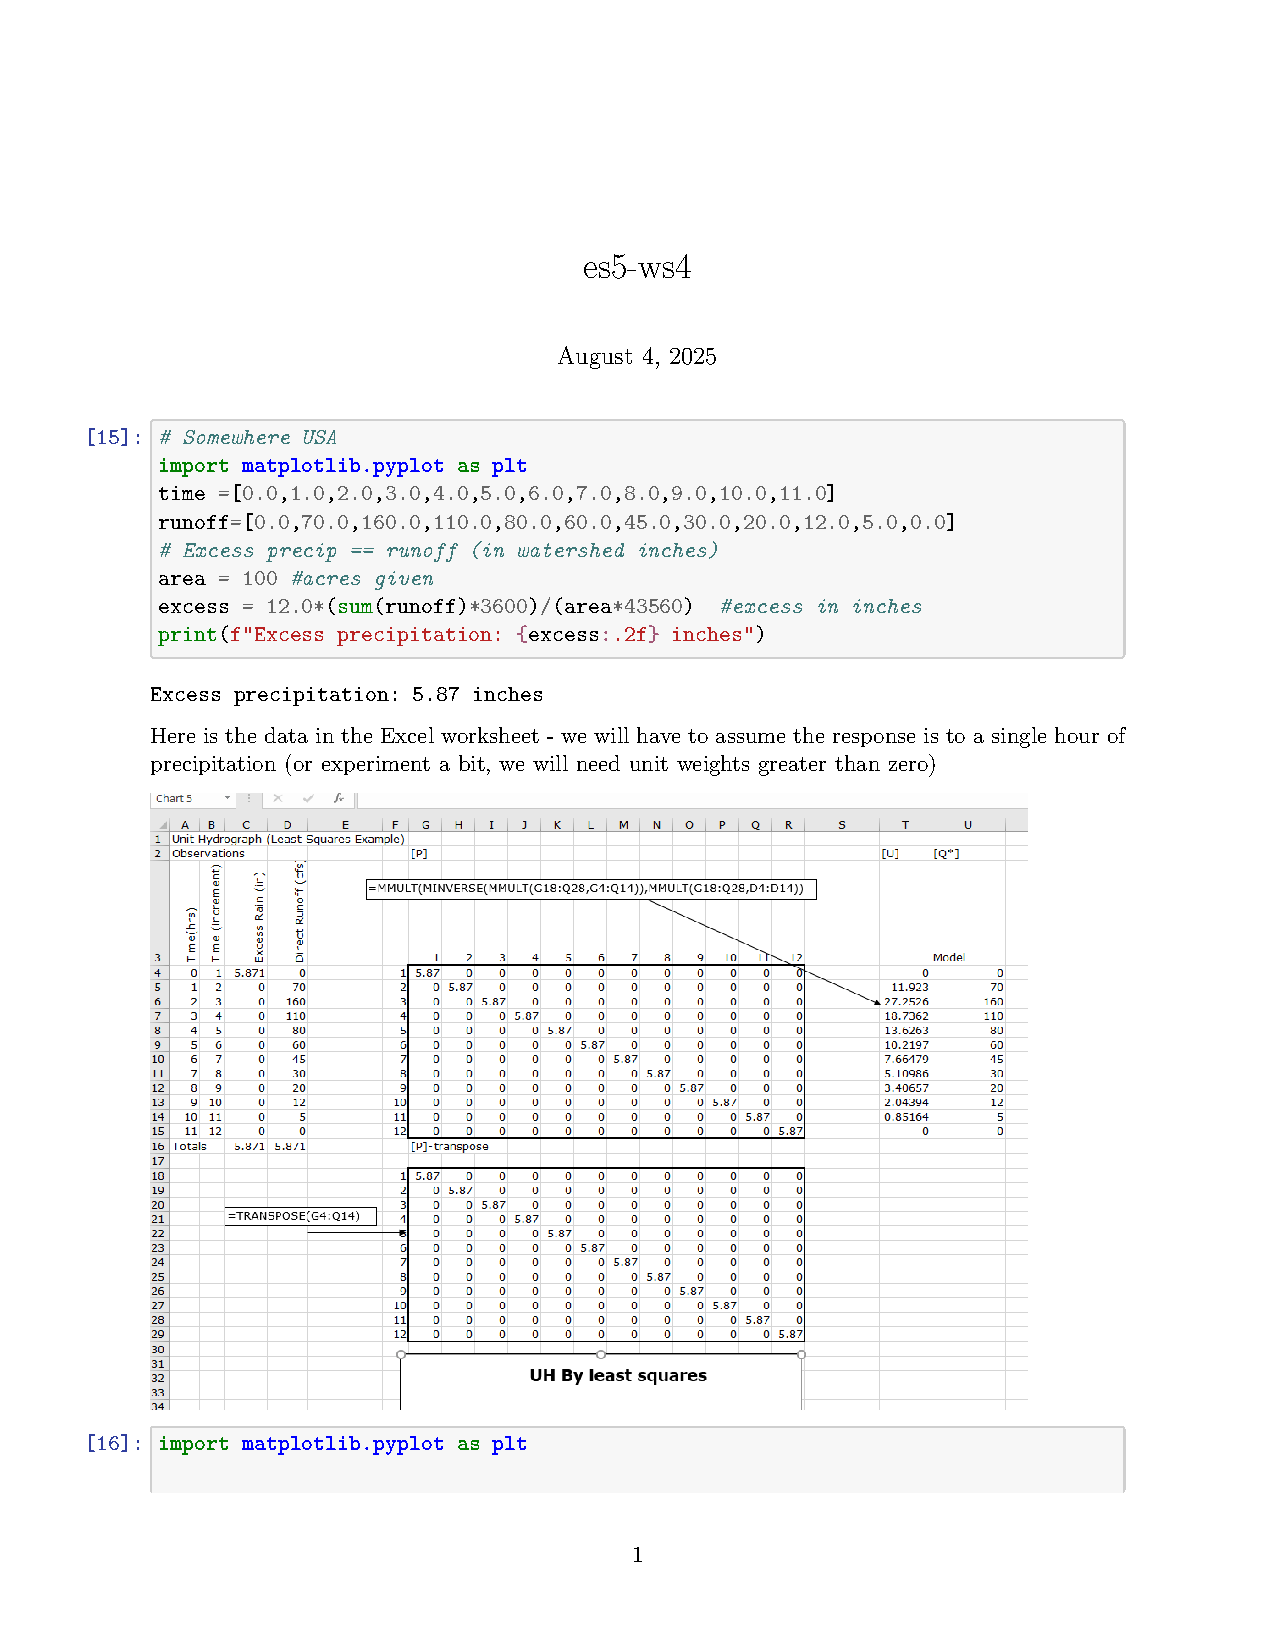
\includepdf[pages=-]{es5-ws4.pdf}

\clearpage

%\item Problem 7.3.5 in Mays, pg. 278.

\item An agricultural watershed was urbanized over a 20 year interval.  A triangular one-hour unit hydrograph was developed for this watershed for an excess rainfall duration of one hour.  

Before urbanization, the average loss rate was 0.30 in/hr.  

Figure \ref{fig:UnitGraph1} is the unit hydrograph that has a peak discharge of 400 cfs/in occurring at 3 hours, and a base time of 9 hours.
\begin{figure}[h!] %  figure placement: here, top, bottom, or page
   \centering
   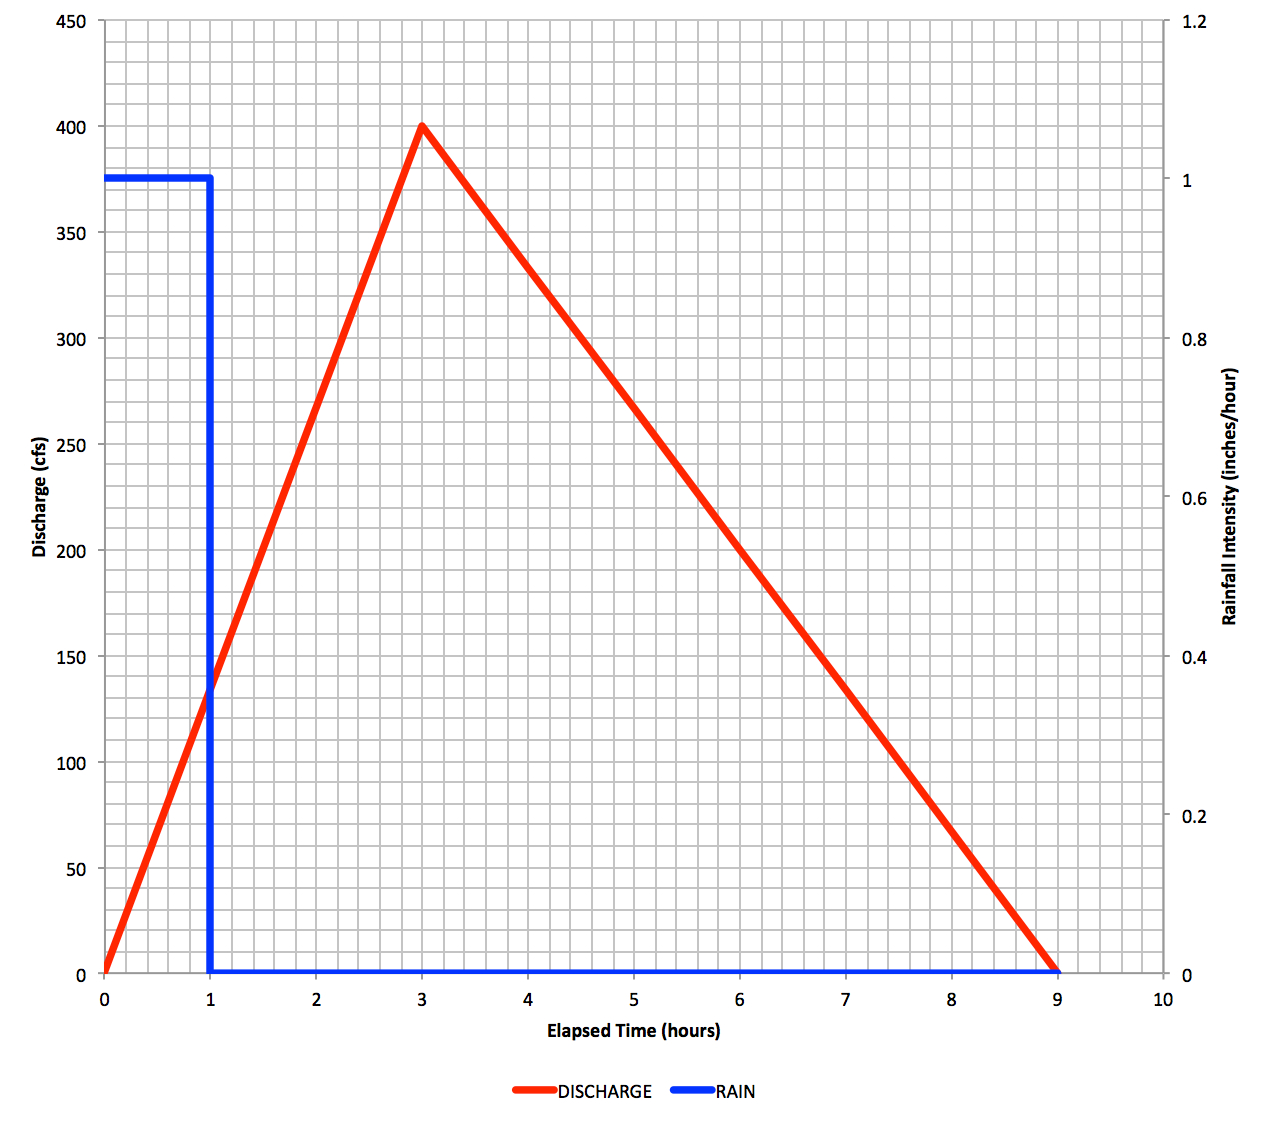
\includegraphics[width=5in]{UnitGraph1.jpg} 
   \caption{Pre-Urbanization unit hydrograph for excess rainfall of 1 in/hr for 1 hour.}
   \label{fig:UnitGraph1}
\end{figure}
\clearpage

After urbanization the loss rate was reduced to 0.15 in/hr and the peak discharge of the unit hydrograph increased to 600 cfs/in occurring at 1 hour, and the base time reduced to 6 hours.    Figure \ref{fig:UnitGraph2} is the unit hydrograph with a peak discharge of 600 cfs occurring at 1 hours, and a time base of 6 hours.

\begin{figure}[h!] %  figure placement: here, top, bottom, or page
   \centering
   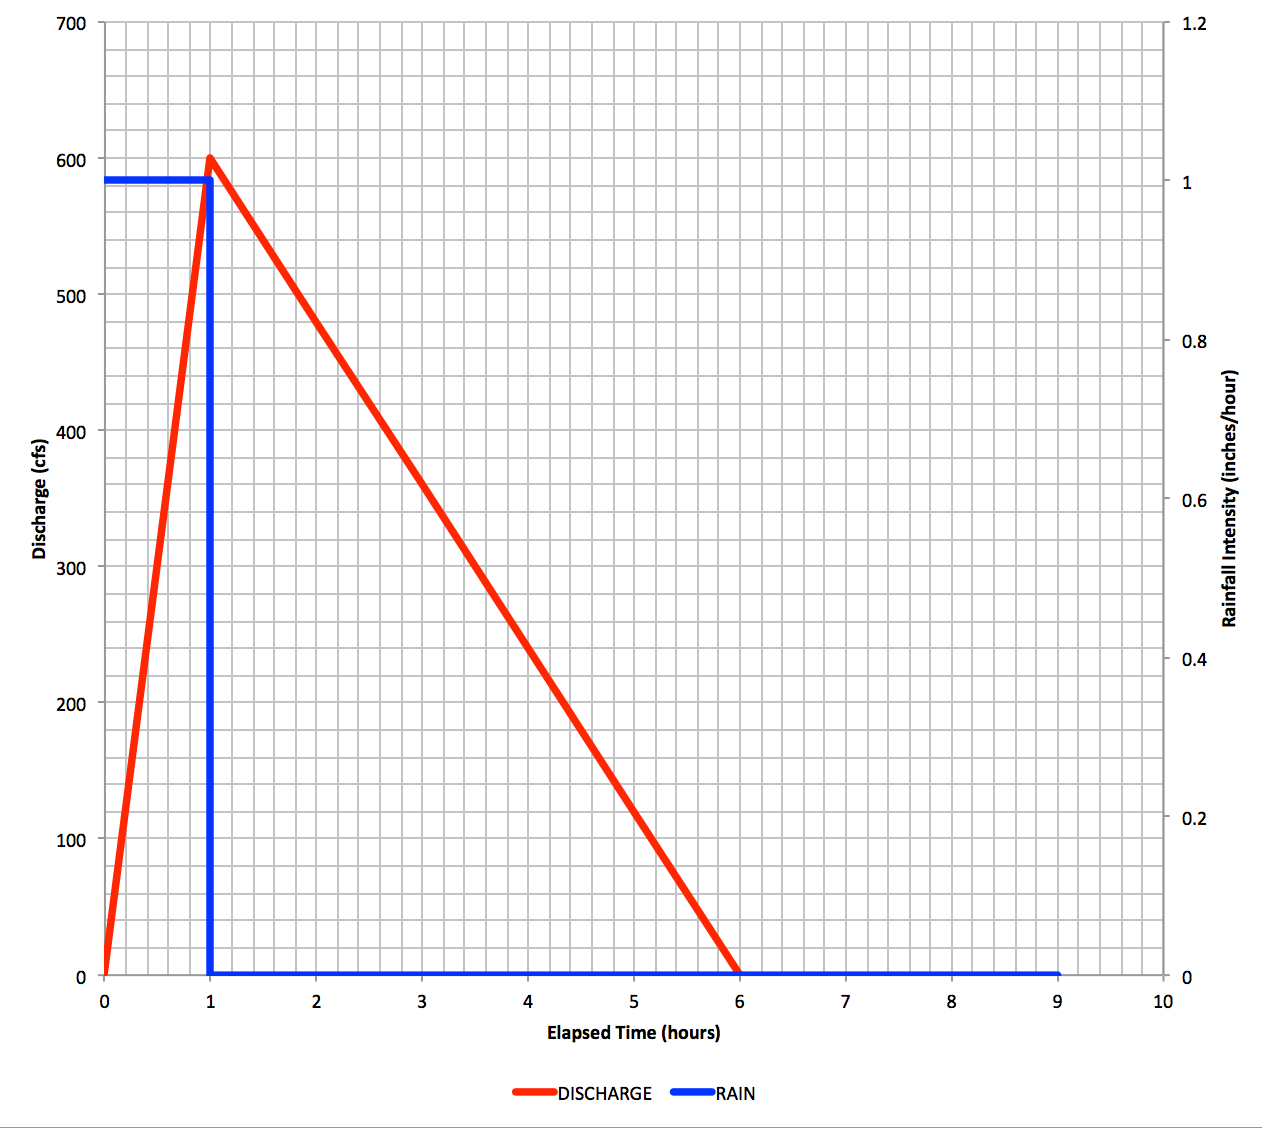
\includegraphics[width=5in]{UnitGraph2.jpg} 
   \caption{Post-Urbanization unit hydrograph for excess rainfall of 1 in/hr for 1 hour.}
   \label{fig:UnitGraph2}
\end{figure}

For a two hour storm in which 1 inch of rain fell in the first hour and 0.5 inch in the second hour, determine the direct runoff hydrographs before and after urbanization.\footnote{This exercise is the same as problem 7.5.7, pg. 238 in Chow, Maidment, Mays}

\clearpage

\textbf{Solution}

\begin{enumerate}[a)]

\item Using Figure \ref{fig:UnitGraph1} as a template, the two increments of rainfall are directly plotted onto the template, then loss is applied to each increment.  The resulting unitgraphs from each increment are plotted (in magenta/purple) and then ordinate-by-ordinate addition is used to construct the composite direct runoff hydrograph, as depicted in Figure \ref{fig:PreUrban}

\begin{figure}[h!] %  figure placement: here, top, bottom, or page
   \centering
   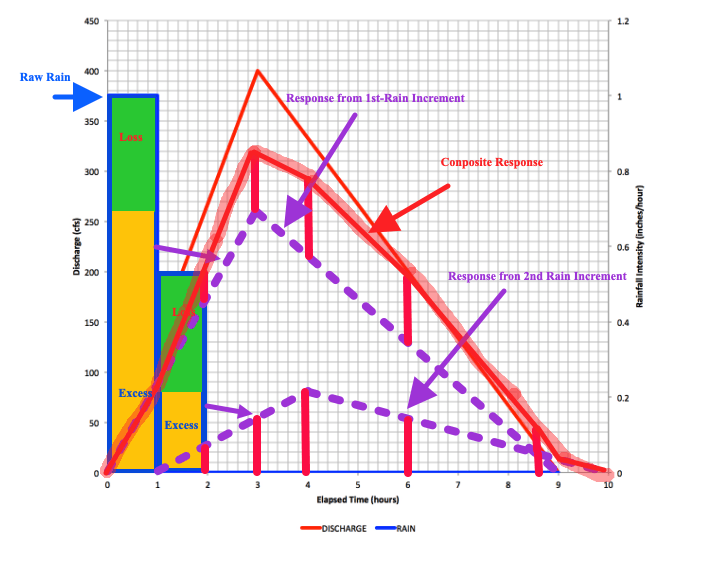
\includegraphics[width=6in]{PreUrban.png} 
   \caption{Pre-Urbanization unit hydrograph for excess rainfall of 1 in/hr for 1 hour.}
   \label{fig:PreUrban}
\end{figure}

\clearpage
%%%%%%%%%%%%%%%%%%%%%%%%%%%%%%%%%

\item Using Figure \ref{fig:UnitGraph2} as a template, the two increments of rainfall are directly plotted onto the template, then loss is applied to each increment.  The resulting unitgraphs from each increment are plotted (in magenta/purple) and thenordinate-by-ordinate addition is used to construct the composite direct runoff hydrograph, as depicted in Figure \ref{fig:PostUrban}

\begin{figure}[h!] %  figure placement: here, top, bottom, or page
   \centering
   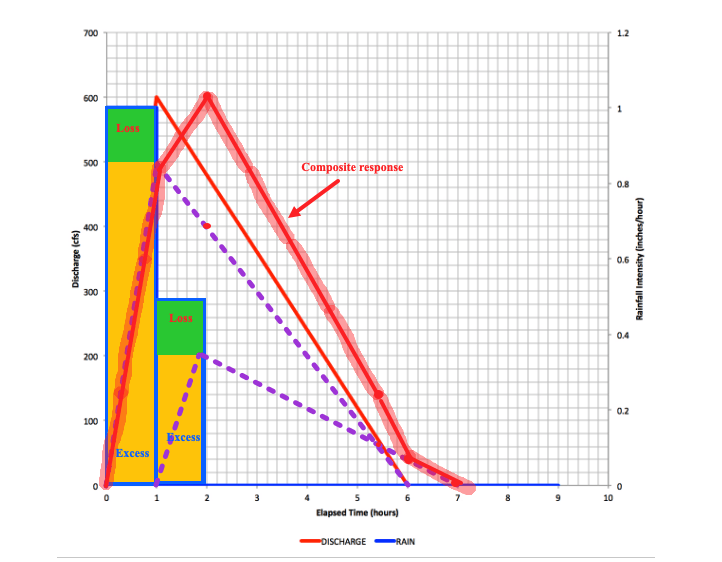
\includegraphics[width=6in]{PostUrban.png} 
   \caption{Post-Urbanization unit hydrograph for excess rainfall of 1 in/hr for 1 hour.}
   \label{fig:PostUrban}
\end{figure}

\clearpage
%%%%%%%%%%%%%%%%%%%%%%%%%%%%%%%%%%%

\item Alternatively (and more usefully) the responses can be incorporated into a spreadsheet as depicted in Figure \ref{fig:UHfromDrawings}.

\begin{figure}[h!] %  figure placement: here, top, bottom, or page
   \centering
   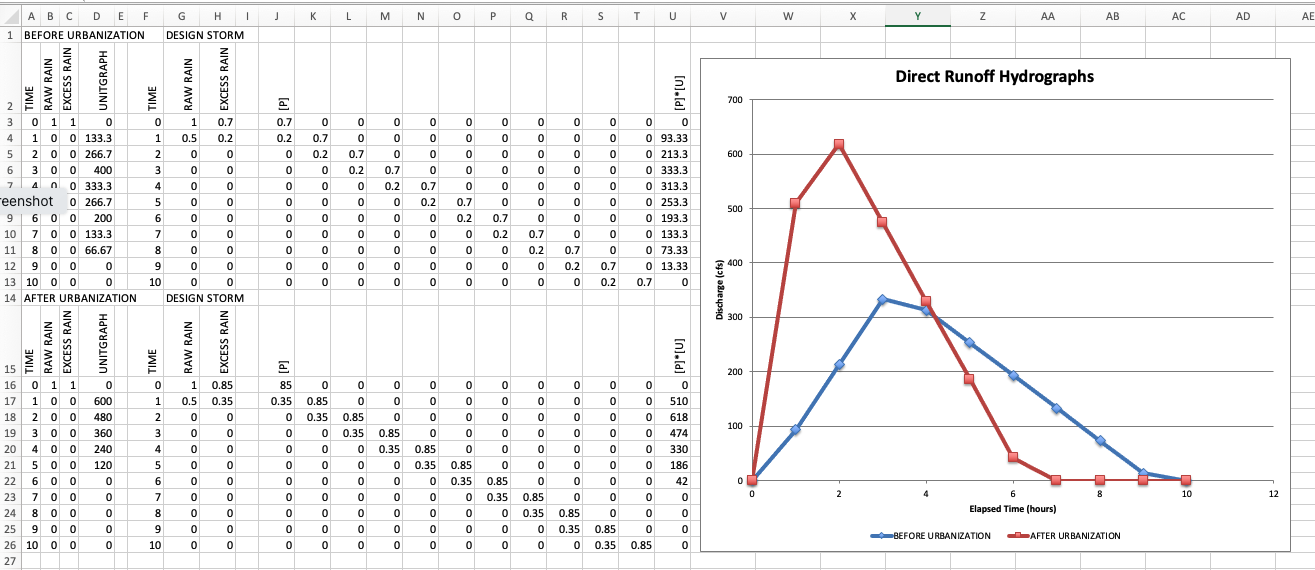
\includegraphics[width=6in]{UHfromDrawings.png} 
   \caption{Spreadsheet solution}
   \label{fig:UHfromDrawings}
\end{figure}

The working spreadsheet is located at \url{http://54.243.252.9/ce-3354-webroot/2-Exercises/ES-6/ES6-SourceCode/ES6-Solution.xlsx}. Figure \ref{fig:UHfromDrawings} is captures from Tab Sheet ``P1.''

\end{enumerate}
\clearpage

\item A storm on April 16, 1977, on the Shoal Creek watershed at Northwest Park in
Austin, Texas, resulted in the rainfall-runoff values in Figure \ref{fig:RainRunoff1}.

Use the linear regression method to determine the half-hour unit hydrograph for the watershed. 
The watershed drainage area is 7.03 $mi^2$.
Assume that a uniform loss rate (constant loss model) is valid.\footnote{This exercise is a hybrid of problems 7.6.2 and 7.6.5, pg  239 in Chow, Maidment, and Mays.}

\begin{figure}[h!] %  figure placement: here, top, bottom, or page
   \centering
   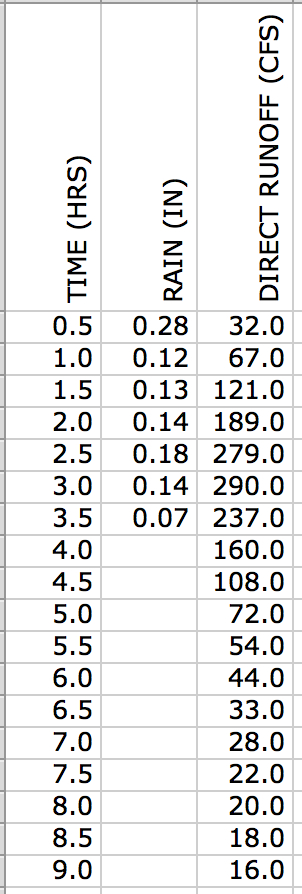
\includegraphics[width=1.5in]{RainRunoff1.jpg} 
   \caption{Observed storm rainfall incremental depths and observed direct runoff hydrograph}
   \label{fig:RainRunoff1}
\end{figure}

\clearpage

%%%%%%%%%%%%%%%%%%%%%%%%%%%%%%%%
\textbf{Solution}

\begin{enumerate}[a)]

\item Using data from Figure \ref{fig:RainRunoff1} and the supplied watershed area, the rainfall is converted into watershed input volume in same units as watershed runoff volume.  A constant loss is applied to the rainfall increments until the ratio of output to input is unity.  as a template, the two increments of rainfall are directly plotted onto the template, then loss is applied to each increment.  Predict-and-correct or Goal Seek is sufficient as depicted in Figure \ref{fig:VolumeBalance}

\begin{figure}[h!] %  figure placement: here, top, bottom, or page
   \centering
   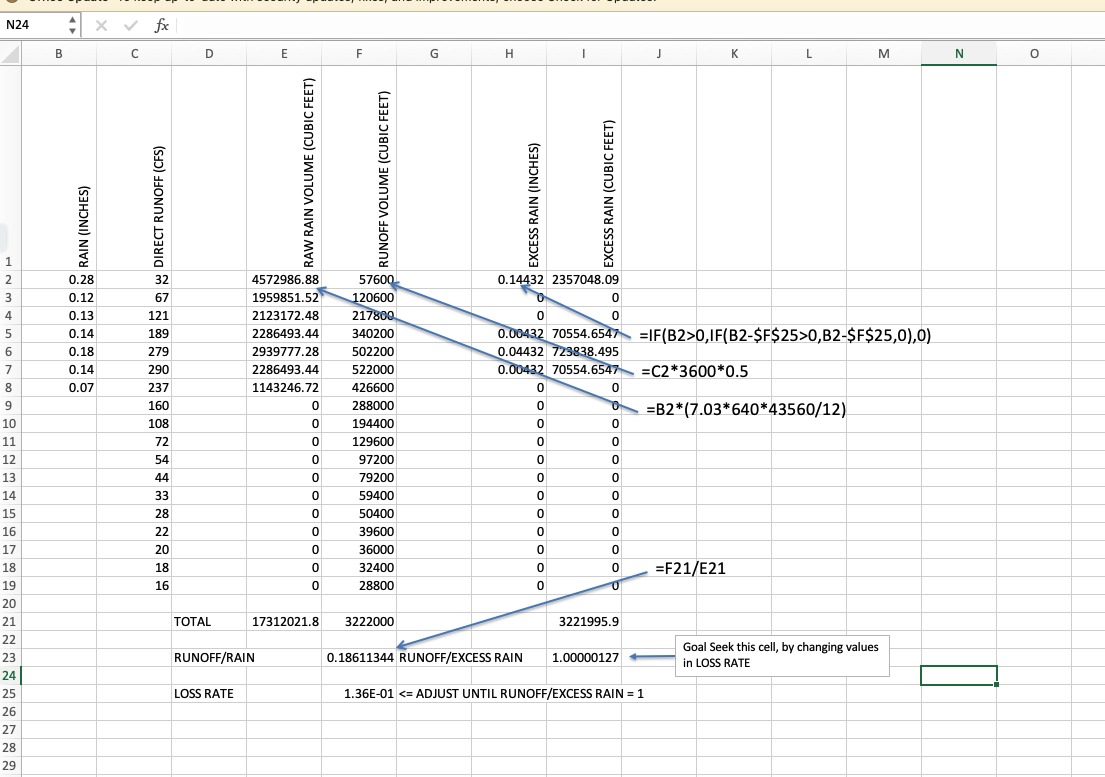
\includegraphics[width=6in]{VolumeBalance.png} 
   \caption{Volume Balance for Shoal Creek data to infer constant loss rate}
   \label{fig:VolumeBalance}
\end{figure}

\clearpage
%%%%%%%%%%%%%%%%%%%%%%%%%%%%%%%%%%%

\item Use the Matrix-Vector representation and ordinary-least-squares to construct a unit hydrograph for the watershed as depicted in Figure \ref{fig:UHbyRegression}.\footnote{This watershed will yield two negative ordinates; a SOLVER result is also shown.  Recall negative ordinates are not physically relevant, and require addressing.  They may simply be artifacts, or (more likely) sample aliasing.}

\begin{figure}[h!] %  figure placement: here, top, bottom, or page
   \centering
   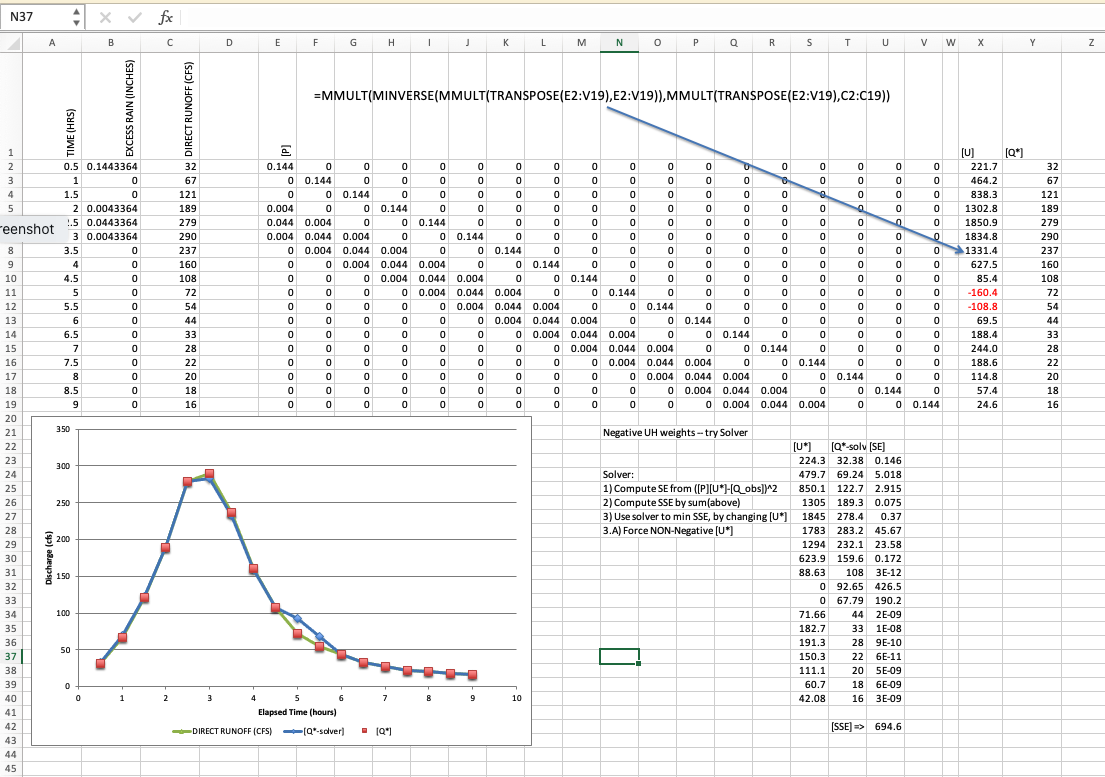
\includegraphics[width=6in]{UHbyRegression.png} 
   \caption{Spreadsheet solution}
   \label{fig:UHbyRegression}
\end{figure}

The working spreadsheet is located at \url{http://54.243.252.9/ce-3354-webroot/2-Exercises/ES-6/ES6-SourceCode/ES6-Solution.xlsx}. Figure \ref{fig:UHfromDrawings} is captured from Tab Sheet ``P2-UH-CL-LOSS-FIT''

\end{enumerate}

\clearpage

\item Table \ref{tab:SomewhereElseUSAUnitgraph} is a 15-minute unit hydrograph for Somewhere Else USA.  Table \ref{tab:SomewhereElseUSAExcessRain} is a precipitation input time-series for the watershed

\begin{table}[h!]
\centering
\caption{Somewhere Else USA Unit Hydrograph Tabulation}
\begin{tabular}{p{2.0in}p{2.0in}} % Column formatting, @{} suppresses leading/trailing space
~&~\\
Time (hours) & Runoff (CFS) \\
\hline
\hline
0.00 & ~~0 \\
0.25 & ~70 \\
0.50 & 182 \\
0.75 & 137 \\
1.00 & ~68 \\
1.25 & ~33 \\
1.50 & ~16 \\
1.75 & ~~9 \\
2.00 & ~~5 \\
2.25 & ~~2 \\
2.50 & ~~1 \\
2.75 & ~0.0 \\
\hline
\end{tabular}
\label{tab:SomewhereElseUSAUnitgraph}
\end{table}

\begin{table}[h!]
\centering
\caption{Somewhere Else USA Excess Rain Input}
\begin{tabular}{p{2.0in}p{2.0in}} % Column formatting, @{} suppresses leading/trailing space
~&~\\
Time (hours) & Rainfall Excess (inches) \\
\hline
\hline
0.00 & ~~0 \\
0.25 & 0.50 \\
0.50 & 1.25 \\
0.75 & 0.75 \\
\hline
\end{tabular}
\label{tab:SomewhereElseUSAExcessRain}
\end{table}

Determine:
    \begin{enumerate}[a)]
        \item The design (direct runoff hydrograph) for the excess rainfall input time series.
        \item A plot of the design hydrograph.
    \end{enumerate}

\textbf{Solution(s):}
Entire problem as Jupyter Notebook (ENGR-1330) on following pages.
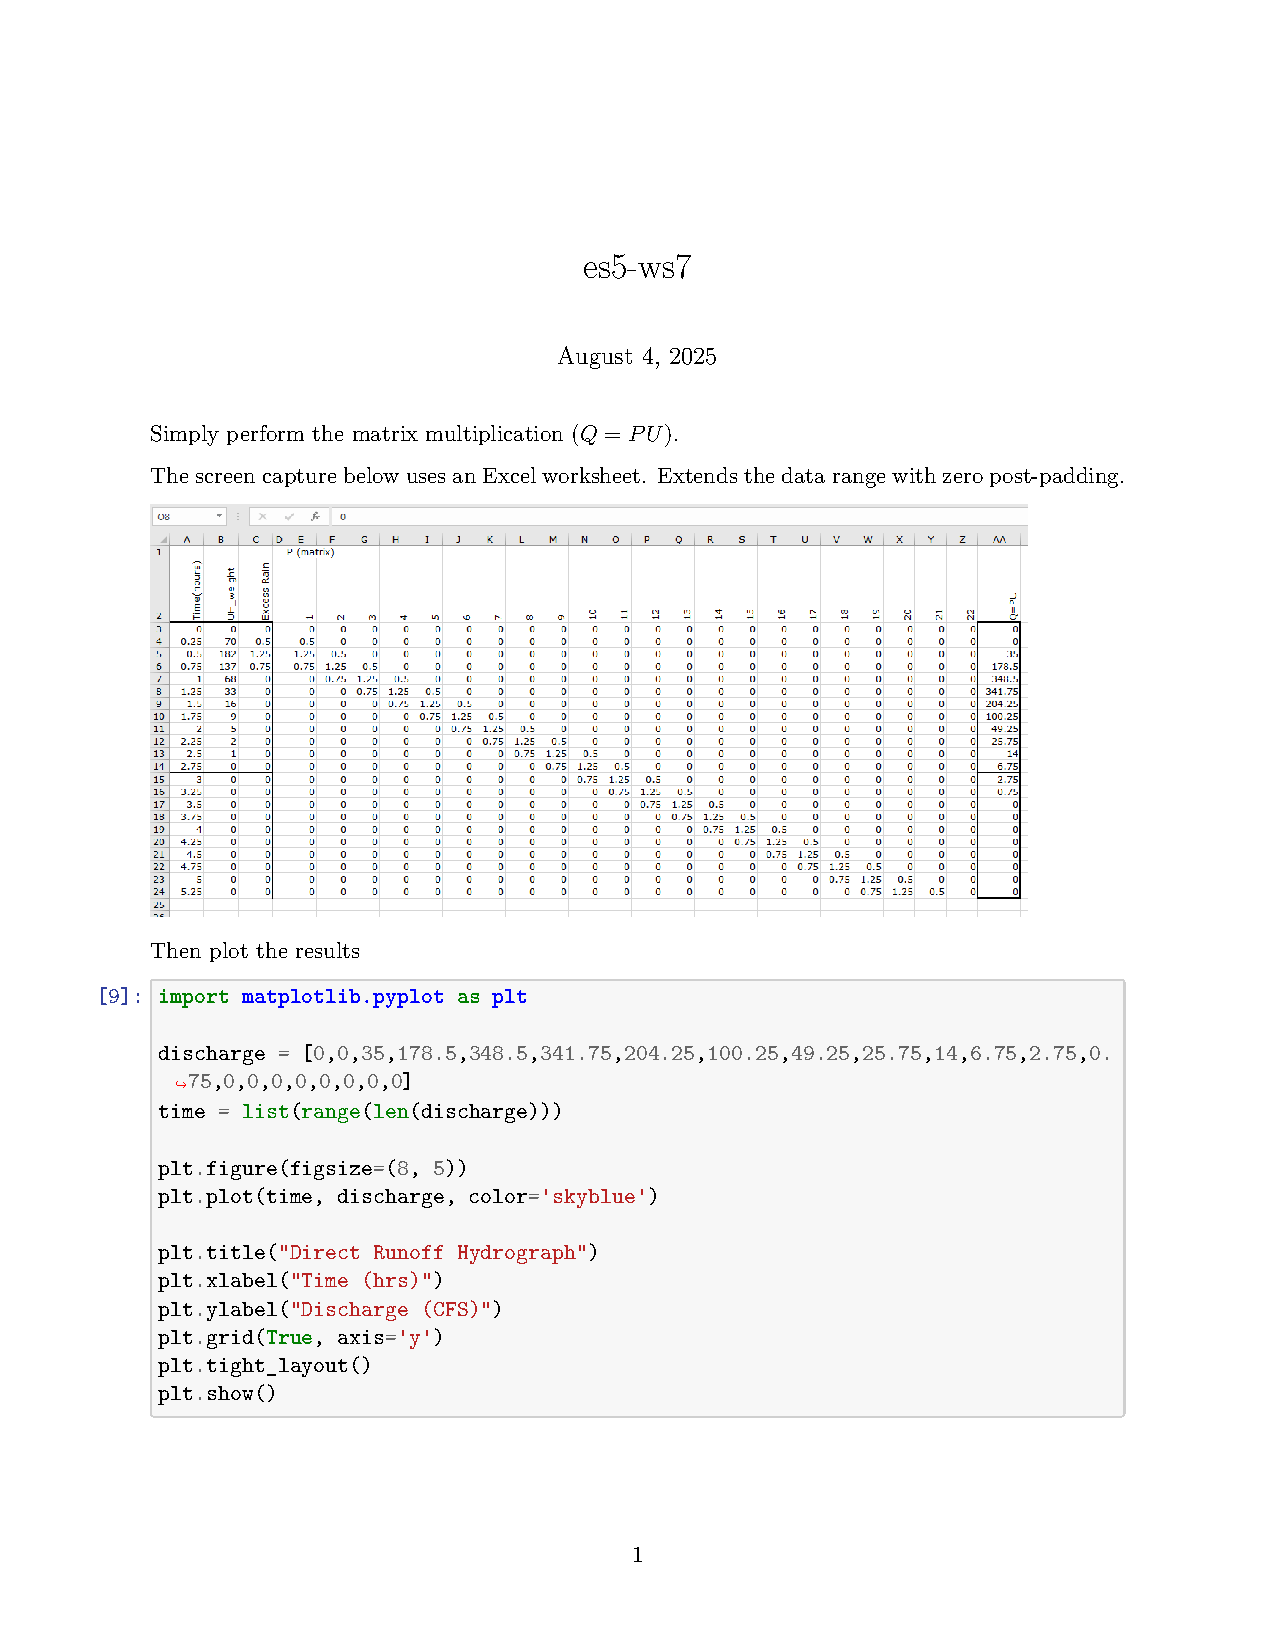
\includepdf[pages=-]{es5-ws7.pdf}

\end{enumerate}

\end{document}  